\subsection{Early days of the Internet and its remaining flaws}\label{early}

The need to build a global communications network in an age when almost nobody had access to that technology and the number of future users was unpredictable, lead to some protocols not being suitable for the huge growth of users that followed. \ac{IPv4} limits the number of public addresses in such a way that today they are scarce \cite{ipv4}. One way to overcome this problem was the development of a mechanism that groups multiple address into a single one, the machine that is assigned that address is then responsible for redirecting messages to members of its group using their private addresses, each connection in the private network is identified publicly by the same \ac{IP} address with a different port.
%RP o porto não identifica uma máquina (membro da rede privada) mas uma ligação.
This technique is known as \ac{NAT}.

\begin{figure}[H]
	\centering
	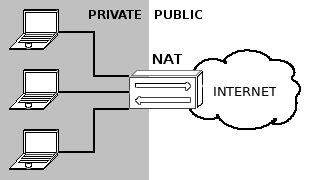
\includegraphics[width=0.6\textwidth]{figures/nat.png}
	\caption{Network Address Translation}
\end{figure}
%RP na figura devias indicar que uns tem ips publicos e outros privados. Alternativamente, colocavas metade da nat box dentro da núvem para indicar que esta pertence à Internet e os pc não. 

Initially \ac{NAT} offered an alternative to address exhaustion and a minimal sensation of security, although its current wide usage, \ac{NAT}s are exposing their weaknesses to the application layer.
%RP initially? E hoje?
There are four types of \ac{NAT} implementations\cite{rfc3489}: \emph{Full Cone NAT}, \emph{Restricted Cone NAT}, \emph{Port Restricted Cone NAT}, \emph{Symmetric NAT}.
%RP apresentas 5. falas em asymmetric. É um erro?

\emph{Full Cone} \ac{NAT} maps each public \ac{IP} address and port to a private \ac{IP} address and port.
Any external host can communicate with private hosts through their mapped public address and port. This represents the least restrictive type of \ac{NAT} and as we will later, the unique type of \ac{NAT} that enables real time communications from point to point.

\emph{Restricted Cone} \ac{NAT} requires that a private client must first send a message to an external host before it can receive messages from the same host. With this type of \ac{NAT}, the private client can be contacted from any port of the same external host.

\emph{Port Restricted Cone} \ac{NAT} works in the same way as Restricted Cone \ac{NAT}, but it only allows communications from the same external host's IP address and port, ignoring all messages from other applications within the same external host.

\emph{Symmetric} NAT maps different ports for each connection, as we will see later, this type of \ac{NAT} represents a problem on real time communications.

\emph{Non-Symmetric} \ac{NAT}s became the common configurations on the Internet. As a direct result, problems started to appear: the amount of ports that \ac{IP} makes available is also small compared to our current needs; worse than that, \ac{NAT} also difficults end-to-end communication, forcing most applications that follow this model to be implemented ineffectively.

Applications behind a \ac{NAT} are prevented to receive incoming connections from the public network, which forces them to behave as a client of a client-server model. 

%RP explicar que o nat funciona num cenário em que a máquina atrás do nat é apenas um consumidor de informação, trabalhando em modo cliente do modelo cliente-servidor. Em P2P isto falha.

Applications based on multimedia and peer-to-peer file sharing have been one of the most strained by \ac{NAT}. Those kind of applications require real time communication in order to achieve the best performance.

\begin{figure}[H]
	\centering
	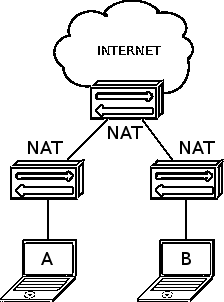
\includegraphics[width=0.25\textwidth]{figures/multinat.png}
	\caption{Multiple level \ac{NAT}s}
\end{figure}

%RP file sharing não precisa de real-time
\ac{STUN} and \ac{TURN} \cite{natvoip} servers are a possible solution to overcome \ac{NAT}, although, none of those can establish direct connections on multiple level \ac{NAT}s.
%HR XXX I was here
%RP explicar o que são multiple level pois não falaste disto antes? São ``nested''?

\ac{STUN} servers are quite simple. They receive requests from \ac{NAT}ed clients, with the source address of a request being the public address that \ac{NAT} mapped to the client. \ac{STUN} servers will then reply to the client, providing the mapped public address, so it knows its associated public \ac{IP} address and port. Symmetric \ac{NAT} changes \ac{IP} port for each different connection, for that reason, when the \ac{STUN} servers reply with the \ac{IP} address and port of their connection, it will be useless for clients to use in other connection connections. That is why Symmetric \ac{NAT} represents a problem for peer-to-peer communications.   
%RP os problemas que relatas têm a ver com P2P ou real-time?

\ac{TURN} uses public servers to relay traffic between private endpoints.
It may use a \ac{P2P} network relay to find the best peer, but after that, the behavior is much like client-server. Direct communication is only achieved by \ac{STUN} when \ac{NAT} is a type \emph{full cone}. \ac{ICE} is a technique that uses \ac{STUN} when direct communications are possible and \ac{TURN} while a direct communication isn't possible.
%RP ainda não explicaste o que é o ICE
%RP explicar que para usar TURN as aplicações têm de estar cientes disso.

Most of client-server applications aren't affected by \ac{NAT} when the servers are public, but they're inadequate for real time communication between two private endpoints. Clearly \ac{TURN} requires a more expensive relaying infrastructure and, in most cases, more network usage, leading to a worse quality of service. The requirements of real-time video communication makes this kind of model unsuitable.
%RP quando falas em infraestrutura mais dispendiosa para o video, está a falar da internet ou ainda estamos a falar de usar ICE?


When connection is established, either in a direct or indirect way (via \ac{TURN} servers), \ac{WebRTC} came to simplify how audio and video are transmitted through web browsers.

\subsection{Real time communications}\label{rtc}

\ac{WebRTC} is an open source technology that defines a collection of standard protocols and JavaScript \ac{API}s for web browser based real time communications without installing any additional application or plug-in. 

Some operating systems such as \emph{Android}, \emph{iOS}, \emph{Linux}, \emph{OSX} and \emph{Windows} implements native \ac{WebRTC} libraries, extending the usage of \ac{WebRTC} to applications outside the web browser. This native support can help to implement applications that record video and audio streams for further playback.

%RP indicar que agora também já temos webrtc fora do browser devido ao seu sucesso e ao facto de reunir tecnologia state of the art?

\begin{figure}[H]
	\centering
	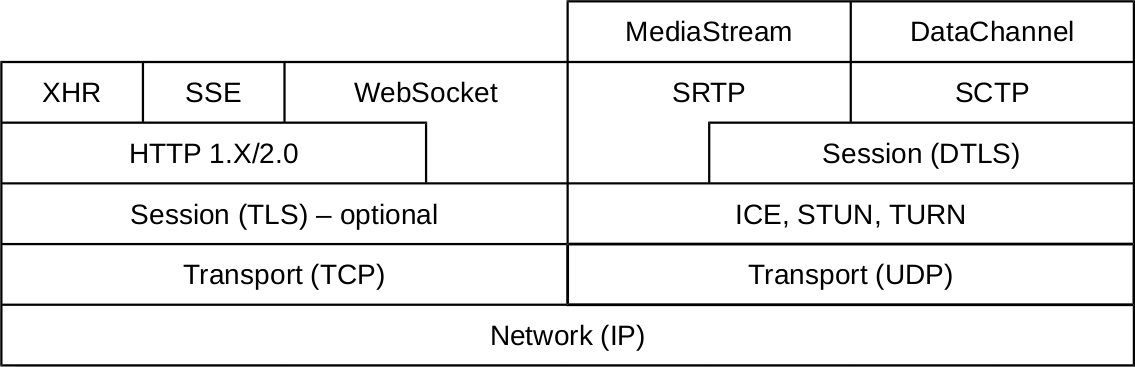
\includegraphics[width=0.9\textwidth]{figures/webrtc_stack.png}
	\caption{WebRTC protocol Stack}
\end{figure}

\ac{WebRTC} defines three main \ac{API}s: MediaStream, PeerConnection and DataChannel. 

\begin{itemize}
  \item \textbf{MediaStream} allows the browser to access the camera, microphone and the device's screen. 

  \item \textbf{PeerConnection} acquires connection data and negotiates with peers.
%RP establishes and negociates a connection with a peer for transmitting real-time video or audio?
  \item \textbf{DataChannel} provides a channel for exchanging arbitrary data with other peers.
\end{itemize}

\ac{WebRTC} uses \ac{UDP} for transporting data, which provides lower latencies than \ac{TCP}, but is not reliable and does not assure packet order and integrity. \ac{SCTP} and \ac{SRTP} are used for streaming data, providing a mechanism for congestion control and partial reliable delivery over \ac{UDP}. All transferred audio, data and video must be encrypted with \ac{DTLS} symmetric keys. \ac{DTLS} provides the same security guarantees as \ac{TLS}. 

\ac{TLS} doesn't support independent record decryption, for that it requires a reliable transport channel, typically \ac{TCP}. The decryption of a record depends on the previous record, which for unreliable transport protocols like \ac{UDP} may represent a problem, either due to packet loss or different reception order.

\ac{DTLS} is similar to \ac{TLS}, but is used on top of \ac{UDP}.
The main difference is the inclusion of a sequence number per packet that is used for packet re-ordering on reception and protects from duplicated packets. If a packet sequence number is less than the expected sequence number the packet is discarded. If a packet sequence number is greater than the expected sequence number the packet may be enqueued or discarded. By knowing the sequence of messages that are sent and received in \ac{DTLS}, timers are used for packet retransmission avoiding acknowledgment messages.
%RP TLS?

\begin{figure}[H]
	\centering
	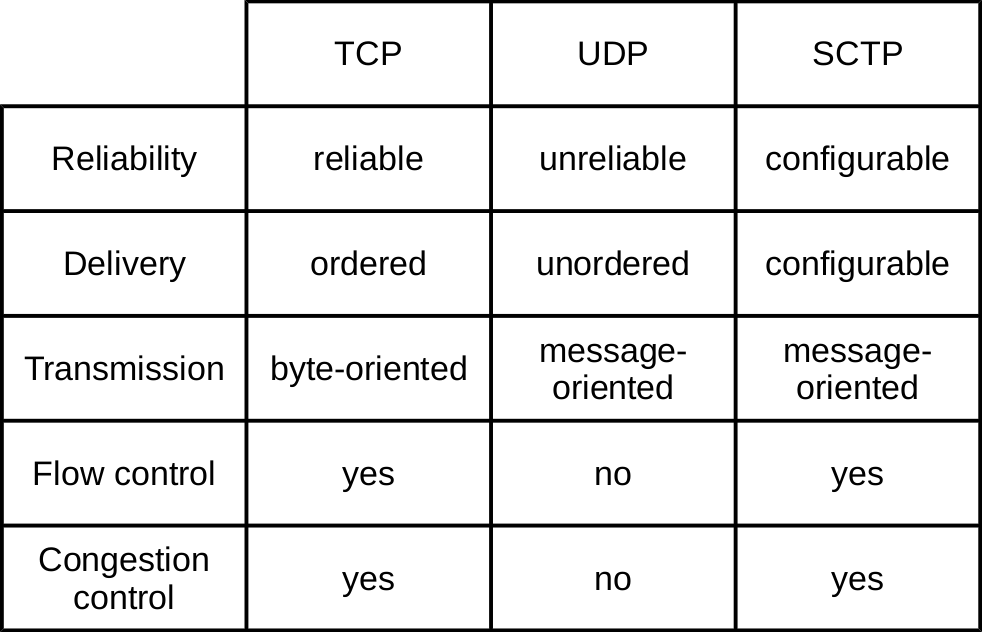
\includegraphics[width=0.6\textwidth]{figures/basic_protocols.png}
	\caption{Overview of transport protocols}
\end{figure}

\ac{WebRTC}'s \emph{DataChannel} is built on top of \ac{SCTP}, which is encapsulated by \ac{DTLS}. \ac{DTLS} encapsulation provides confidentiality, authentication and integrity to the transfered data. A \emph{Data Channel} has one incoming stream and one outgoing stream, providing bidirectional communication. Each data channel direction can be configured for reliable or unreliable transmission, the same can be done for order delivery and priority. which can also be defined for improving the quality of service of a particular stream over the others.

\ac{WebRTC}'s \emph{MediaStream} is built on top of \ac{SRTP}, which requires an external mechanism for key exchange. \ac{DTLS} keys are negotiated on handshake in order to achieve a secure connection. The new keys derived from \ac{DTLS} handshake are seized for \ac{SRTP} encryption, the remaining \ac{SRTP} communications are done through \ac{UDP} without using \ac{DTLS}.
%RP quais remaining?  A última frase é confusa

\ac{WebRTC} aims to provide a standard platform for real-time audio and video on the Web. It arrives at a time when several proprietary products are well established.
\emph{Skype}\footnote{\url{http://www.skype.com/}} is an application that allows video, voice, instant messaging and multi-party communication over proprietary protocols, its main strength are the amount of users that are using it nowadays and the ability to perform voice calls to the \ac{PSTN}. But compared to \emph{Skype}, \ac{WebRTC} applications don't need to be pre-installed.

\emph{Google Hangouts}\footnote{\url{http://plus.google.com/hangouts}} is another popular video multi-party conference web application. 
In the past, in order to use \emph{hangouts} on a web browser a plug-in had to be installed, nowadays hangouts is using \ac{WebRTC}. \emph{Google Hangouts} supports viewing videos on \emph{youtube} synchronously, drawing collaboratively, creating music and playing multi-player games. These applications are implemented with \emph{Adobe Flash}.  

\emph{Jitsi Meet}\footnote{\url{http://jitsi.org/Projects/JitsiMeet}} is a \ac{WebRTC} collaborative application that uses \emph{Jitsi Videobridge} for high quality and scalable video conferences and supports shared document editing. \emph{Jitsi Meet} allows a great amount of users in the same conversation by identifying the current most active participant users and, by consequence, reducing the video and audio quality for all the other users. \emph{Jitsi Videobridge} is a server that enables multi-party video calls. 

%RP a descricção do skype, hangouts e jistsi cai um pouco do céu. Não há uma transição e não é feita uma análise. Apenas são indicados. Não há comparação entre eles nem com o que pode ser feito por webrtc.


